\section{Methodology}
\label{sec:method}

\ours addresses the challenge of PDE discovery through a three-agent closed-loop architecture (Figure \ref{fig:framework}). The \textbf{Symbolic Proposer} (an LLM) generates candidate equation structures by leveraging its pre-trained knowledge of mathematical forms. The \textbf{Numerical Evaluator} fits coefficients to each candidate and computes a fitness score measuring how well the equation explains the observed data. The \textbf{Prompt Optimizer} (a Bayesian Optimization agent) analyzes feedback from the evaluator and selects the optimal instruction strategy for the next generation round. This closed-loop design allows the system to adaptively refine its search strategy based on accumulated evidence, rather than relying on a fixed generation policy.

\paragraph{Dynamic Prompt Construction} The key innovation of our framework is treating the LLM's instruction as a dynamic, optimizable component. Instead of using a static prompt string throughout the discovery process, we dynamically assemble the prompt $P_t$ at each iteration $t$:
\begin{equation}
    P_t = I_{\text{task}} \oplus \mathcal{H}_{\text{top}} \oplus I_{\text{strategy}}^{(k_t)}
\end{equation}
where $\oplus$ denotes string concatenation. Each component serves a distinct purpose: (1) \textbf{Static Context} ($I_{\text{task}}$): This fixed preamble defines the problem setting, including the state variables (e.g., $u, x, t$), the admissible operator library (e.g., $\{+, \times, \partial_x, \partial_{xx}, \sin, \exp\}$), and output formatting requirements. This ensures the LLM understands the symbolic constraints of the task. (2) \textbf{Dynamic Memory} ($\mathcal{H}_{\text{top}}$): To enable learning from past iterations, we include the top-$N$ best-performing equations discovered so far, along with their fitness scores. This in-context history provides the LLM with implicit ``gradient'' information---by observing which structural patterns achieve high scores, the model can identify promising directions for further exploration. (3) \textbf{Optimizable Instruction} ($I_{\text{strategy}}^{(k_t)}$): This is the core optimizable component. Rather than using a generic directive like ``find the best equation,'' we select a specific reasoning strategy from a pre-constructed \textit{Strategy Bank}~\citep{zhou2023ape,sun2024ease} $\mathcal{B} = \{s_1, \ldots, s_K\}$. We generate $K=100$ diverse instruction variants using a meta-LLM (GPT-4o), covering different aspects of the discovery process. These strategies span a spectrum from \textit{exploration} (``Ignore previous bests. Propose a completely new mathematical structure that has not been tried.'') to \textit{parsimony} (``The current best equations are too complex. Identify and remove terms that contribute least to the fit.''), and include \textit{mutation} directives (``Keep the core structure of the best equation but replace the nonlinear interaction terms with alternatives.'') as well as \textit{refinement} instructions (``The structure looks correct. Focus on adjusting the functional form of individual terms.'').


\paragraph{Bayesian Optimization for Strategy Selection} Selecting the optimal strategy at each iteration is itself an optimization problem. However, evaluating any strategy is expensive: it requires generating candidates from the LLM, fitting their coefficients, and computing residuals against the data. This rules out gradient-based or exhaustive search methods.
We model the mapping from strategy index $k \in \{1, \ldots, K\}$ to the resulting best equation fitness as a black-box function $f: \{1,\ldots,K\} \rightarrow \mathbb{R}$. A Gaussian Process surrogate $\mathcal{GP}$ is fitted to the history of (strategy, fitness) pairs observed so far, providing posterior estimates of the mean $\mu(k)$ and uncertainty $\sigma(k)$ for each strategy. We select the next strategy by maximizing the Expected Improvement (EI) acquisition function:
\begin{equation}
    k_{t+1} = \arg\max_{k} \mathbb{E}_{y \sim \mathcal{GP}}\left[\max(y - y^*, 0)\right]
\end{equation}
where $y^*$ is the best fitness score observed so far. EI quantifies the expected gain from trying strategy $k$: it assigns high values to strategies that either have high predicted performance (exploitation) or high uncertainty (exploration). This principled balance allows the system to efficiently navigate the discrete strategy~\citep{baptista2018bocs} space without exhaustively trying all options.

\paragraph{Numerical Evaluation with Parsimony Penalty} Once the LLM generates candidate symbolic skeletons, we must evaluate their quality. Each candidate is parsed into a symbolic expression, and its free coefficients are optimized using sparse regression (specifically, STRidge) ~\citep{tibshirani1996lasso} to minimize the residual against the observed data $\mathcal{D}$. To prevent overfitting through overly complex equations---a common failure mode in symbolic regression---we design a composite fitness function that balances accuracy against parsimony~\citep{bartlett2024mdl,burlacu2019parsimony}:
\begin{equation}
    S(\hat{u}) = \frac{1 - \lambda \cdot \text{complexity}(\hat{u})}{1 + \text{NRMSE}(\hat{u}, \mathcal{D})}
\end{equation}
where $\text{complexity}(\hat{u})$ counts the number of terms in the equation, $\lambda$ is a penalty coefficient (set to 0.01 in our experiments), and NRMSE $= \sqrt{\text{MSE}/\text{Var}(u)}$ is the normalized root mean square error. This formulation ensures that among equations with similar accuracy, simpler ones receive higher scores. A complete algorithmic description with complexity bounds is given in Appendix~\ref{app:algorithm}.

% In document
\begin{figure*}[!htbp]
\centering
\begin{subfigure}{0.33\textwidth}
  \centering
  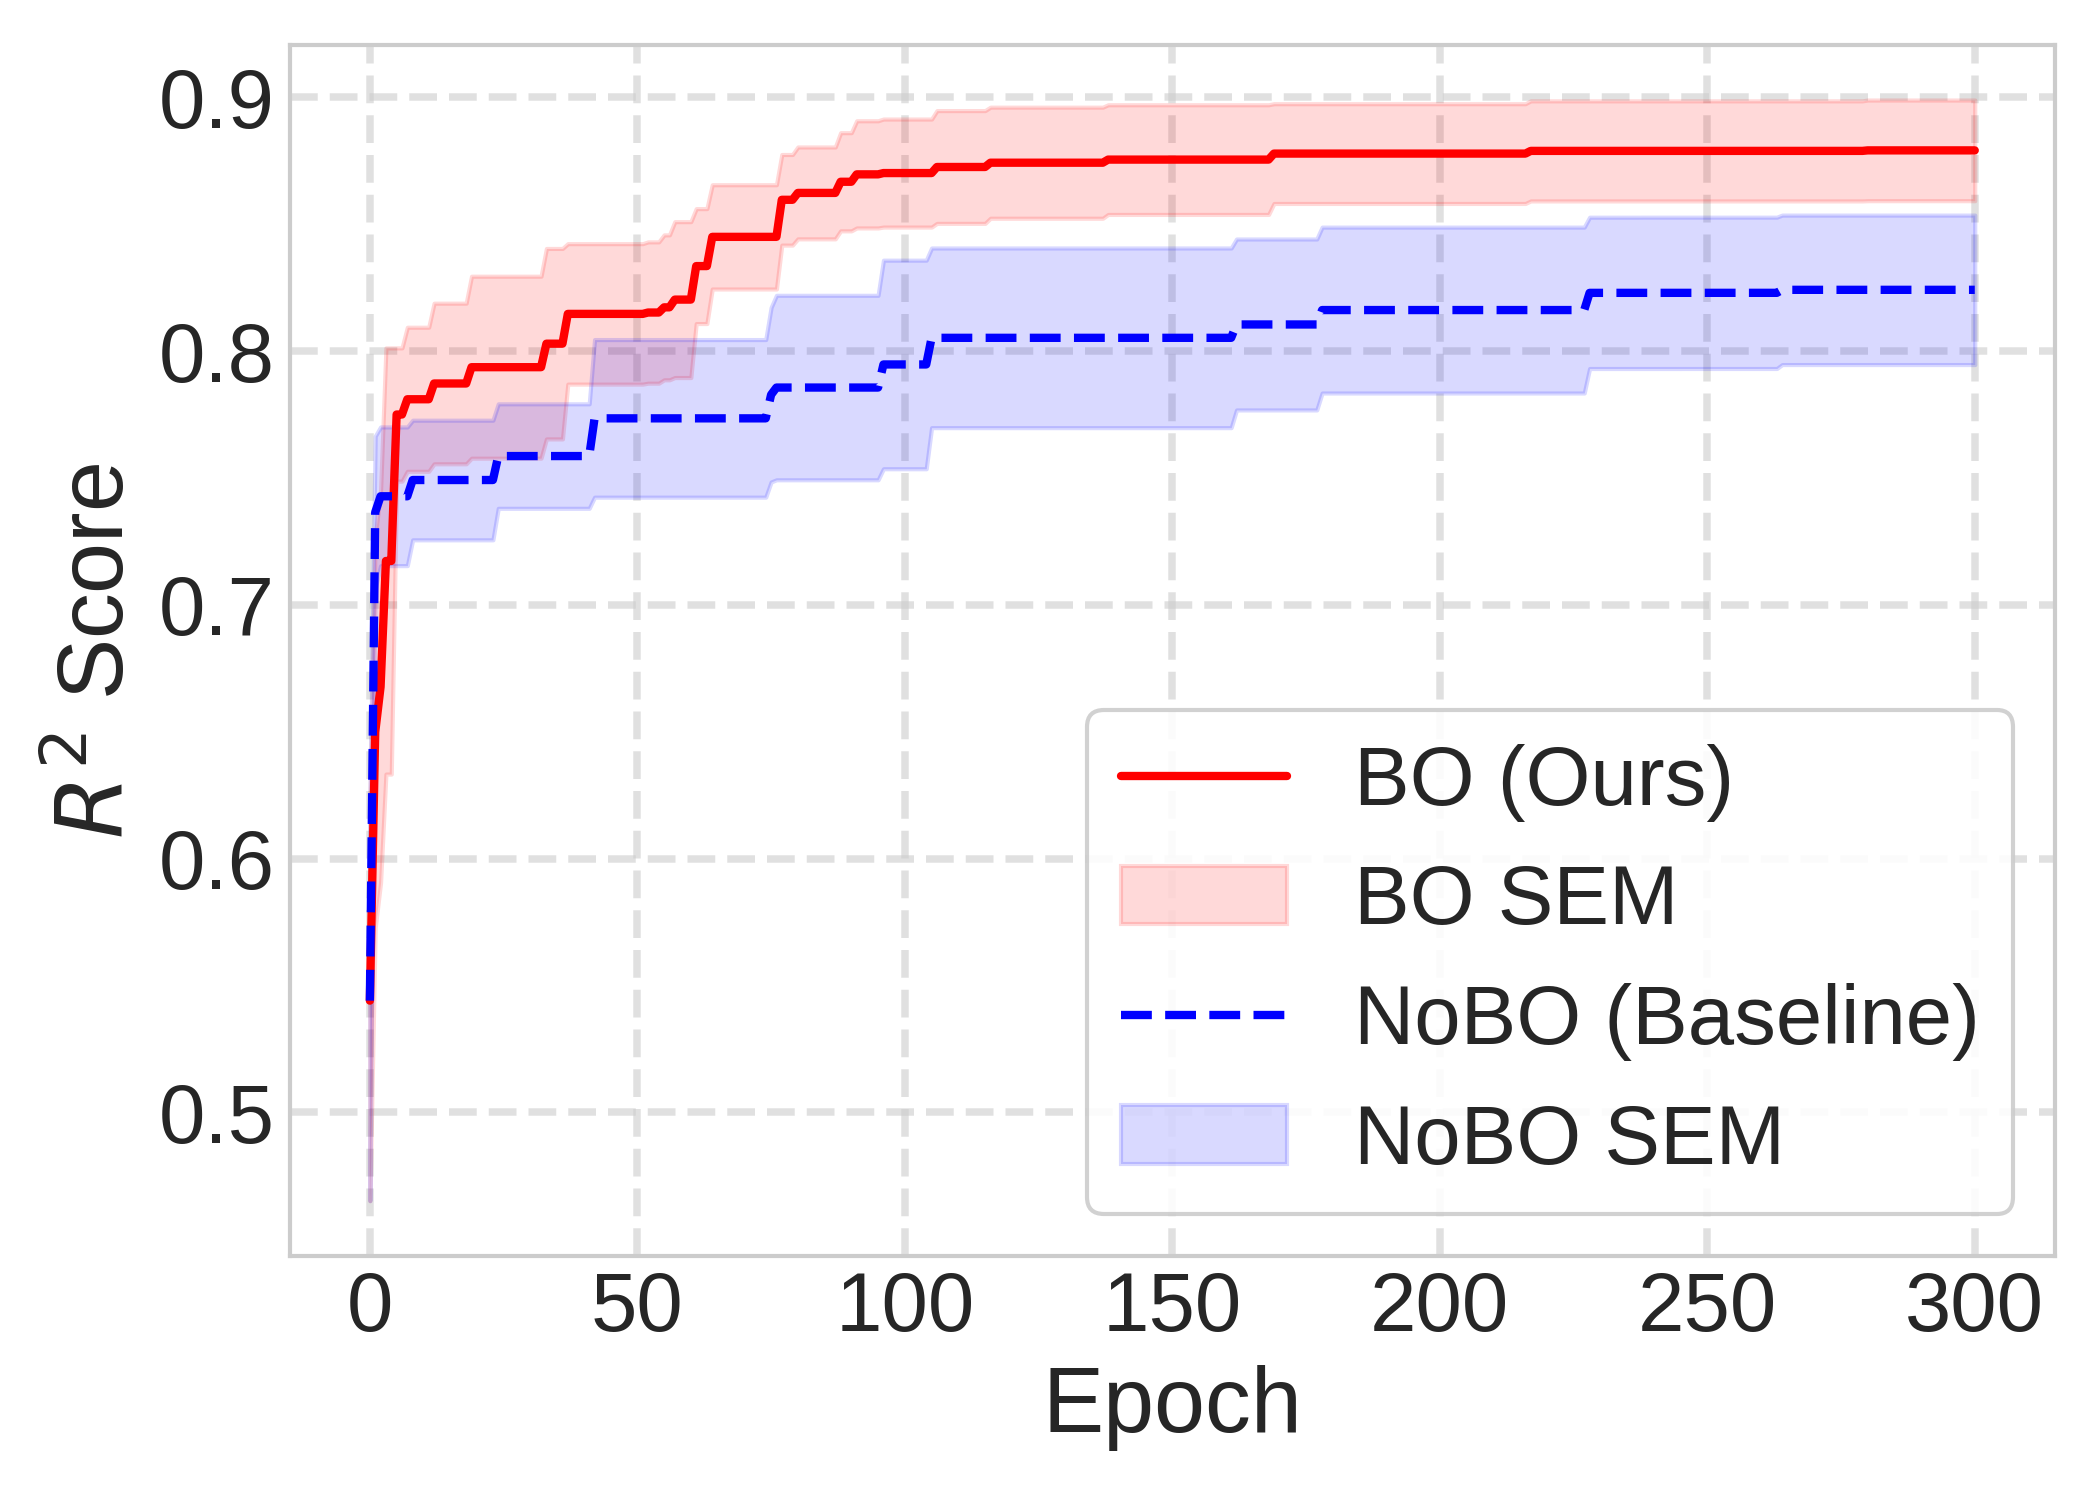
\includegraphics[width=\linewidth]{fig2/Burgers_testing_r2_v1.png}
  \caption{\footnotesize Burgers}
\end{subfigure}\hfill
\begin{subfigure}{0.33\textwidth}
  \centering
  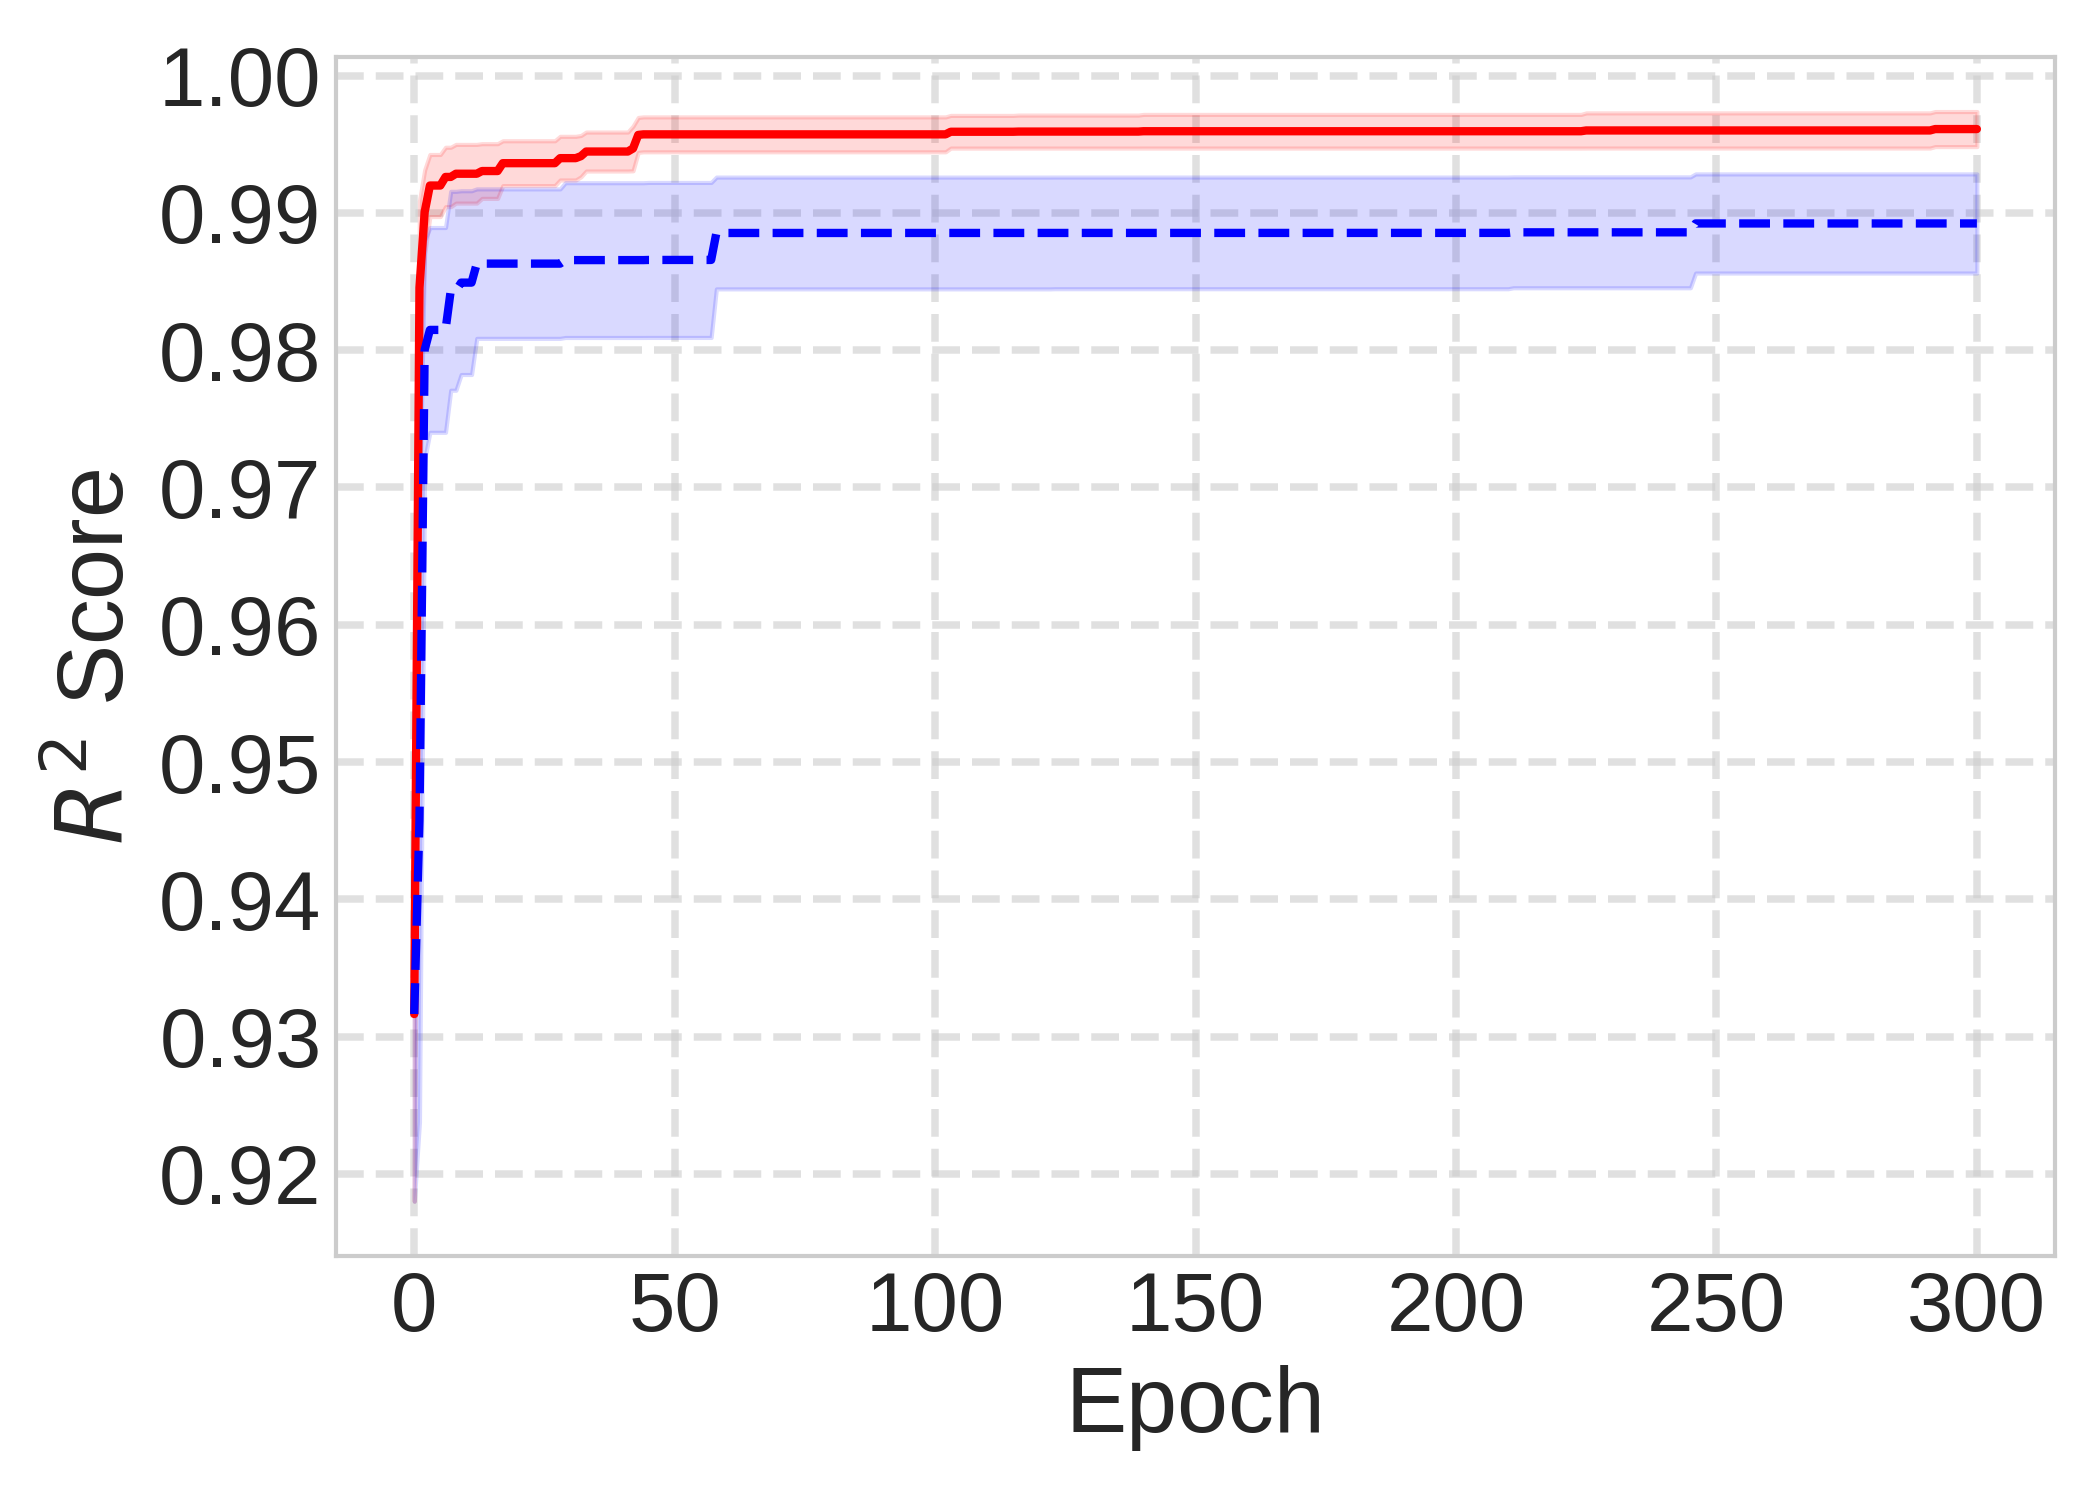
\includegraphics[width=\linewidth]{fig2/Chafee_testing_r2_v1.png}
  \caption{\small Chafee}
\end{subfigure}\hfill
\begin{subfigure}{0.33\textwidth}
  \centering
  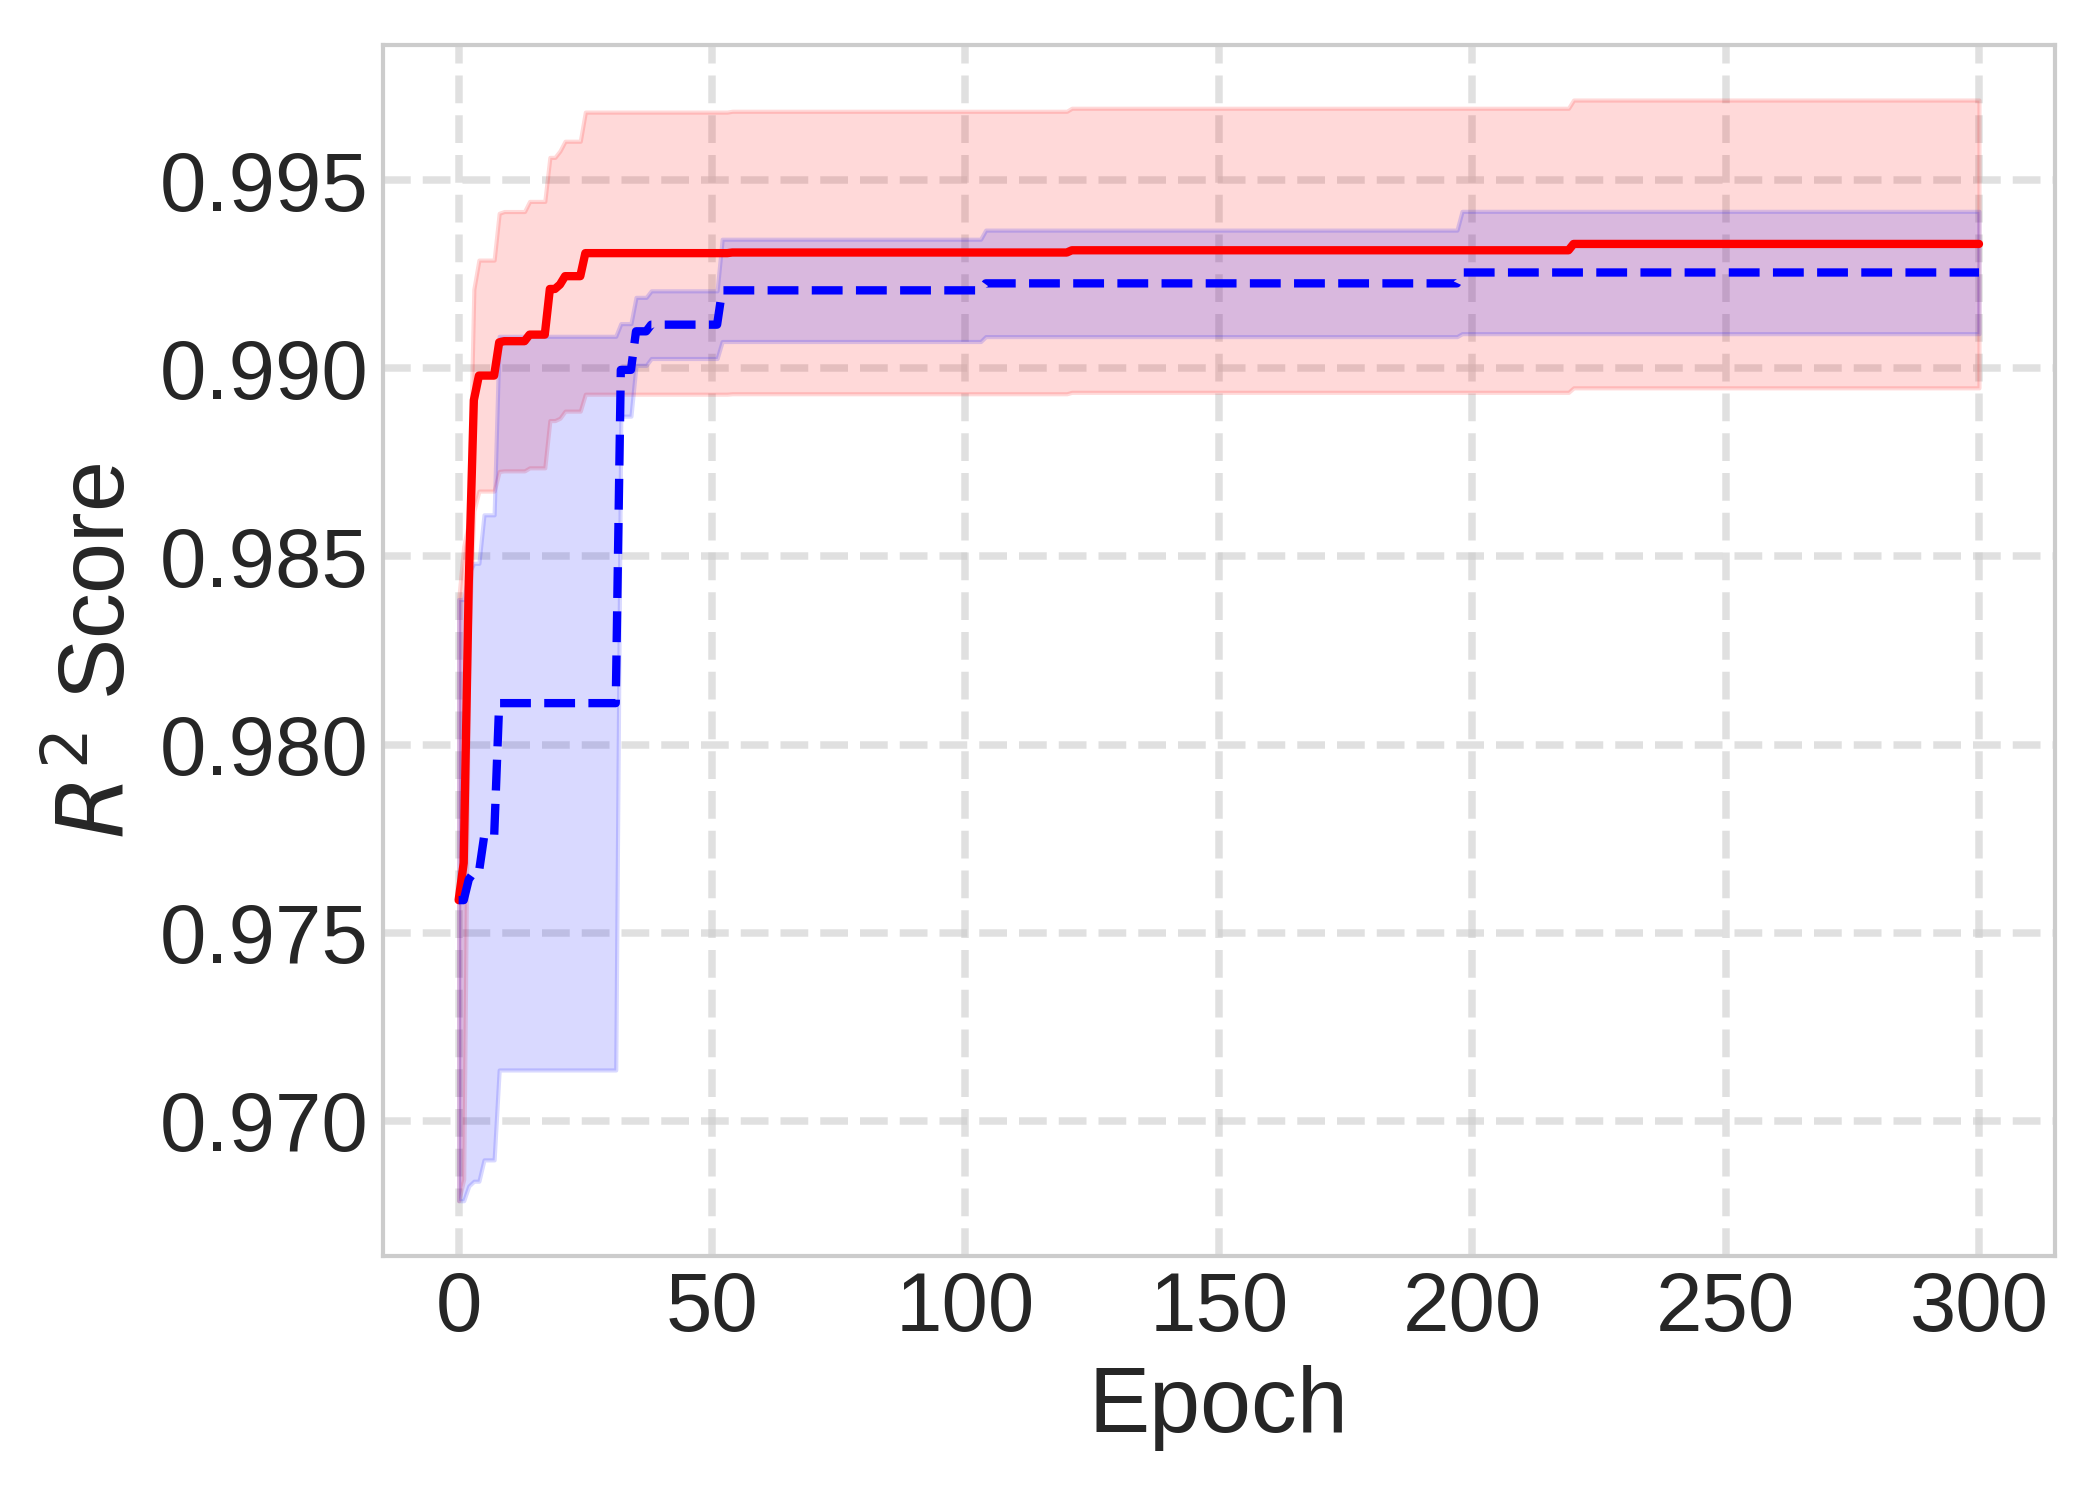
\includegraphics[width=\linewidth]{fig2/Divide_testing_r2_v1.png}
  \caption{\small Divide}
\end{subfigure}\hfill
\\
\begin{subfigure}{0.33\textwidth}
  \centering
  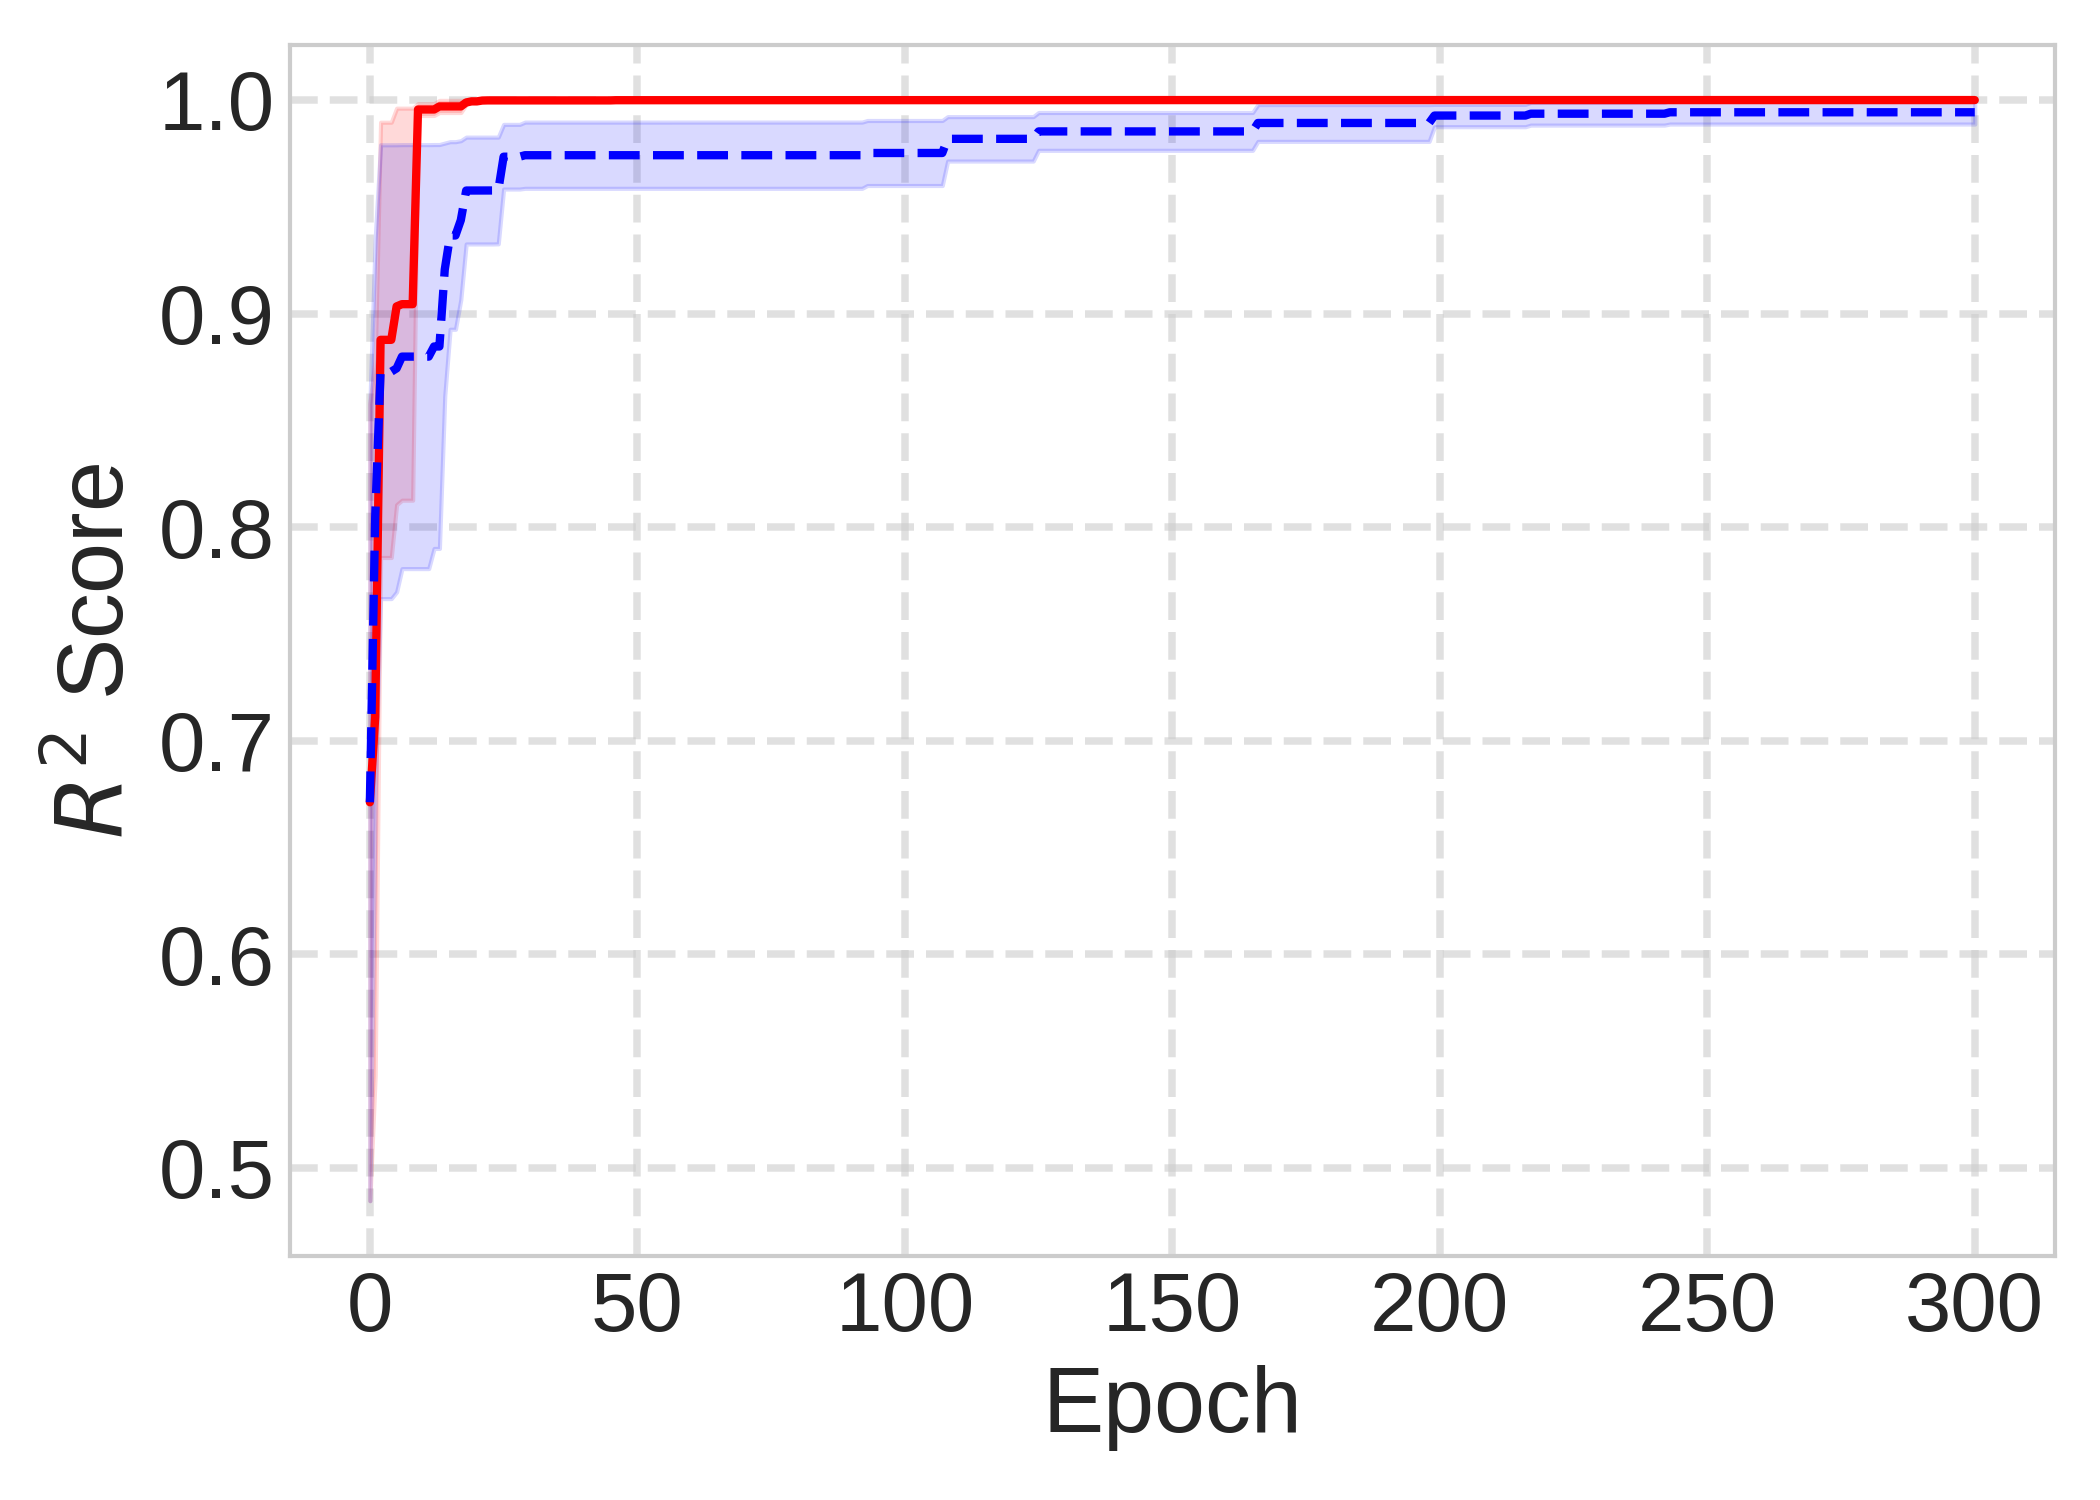
\includegraphics[width=\linewidth]{fig2/Fisher_testing_r2_v1.png}
  \caption{\small Fisher}
\end{subfigure}
\begin{subfigure}{0.33\textwidth}
  \centering
  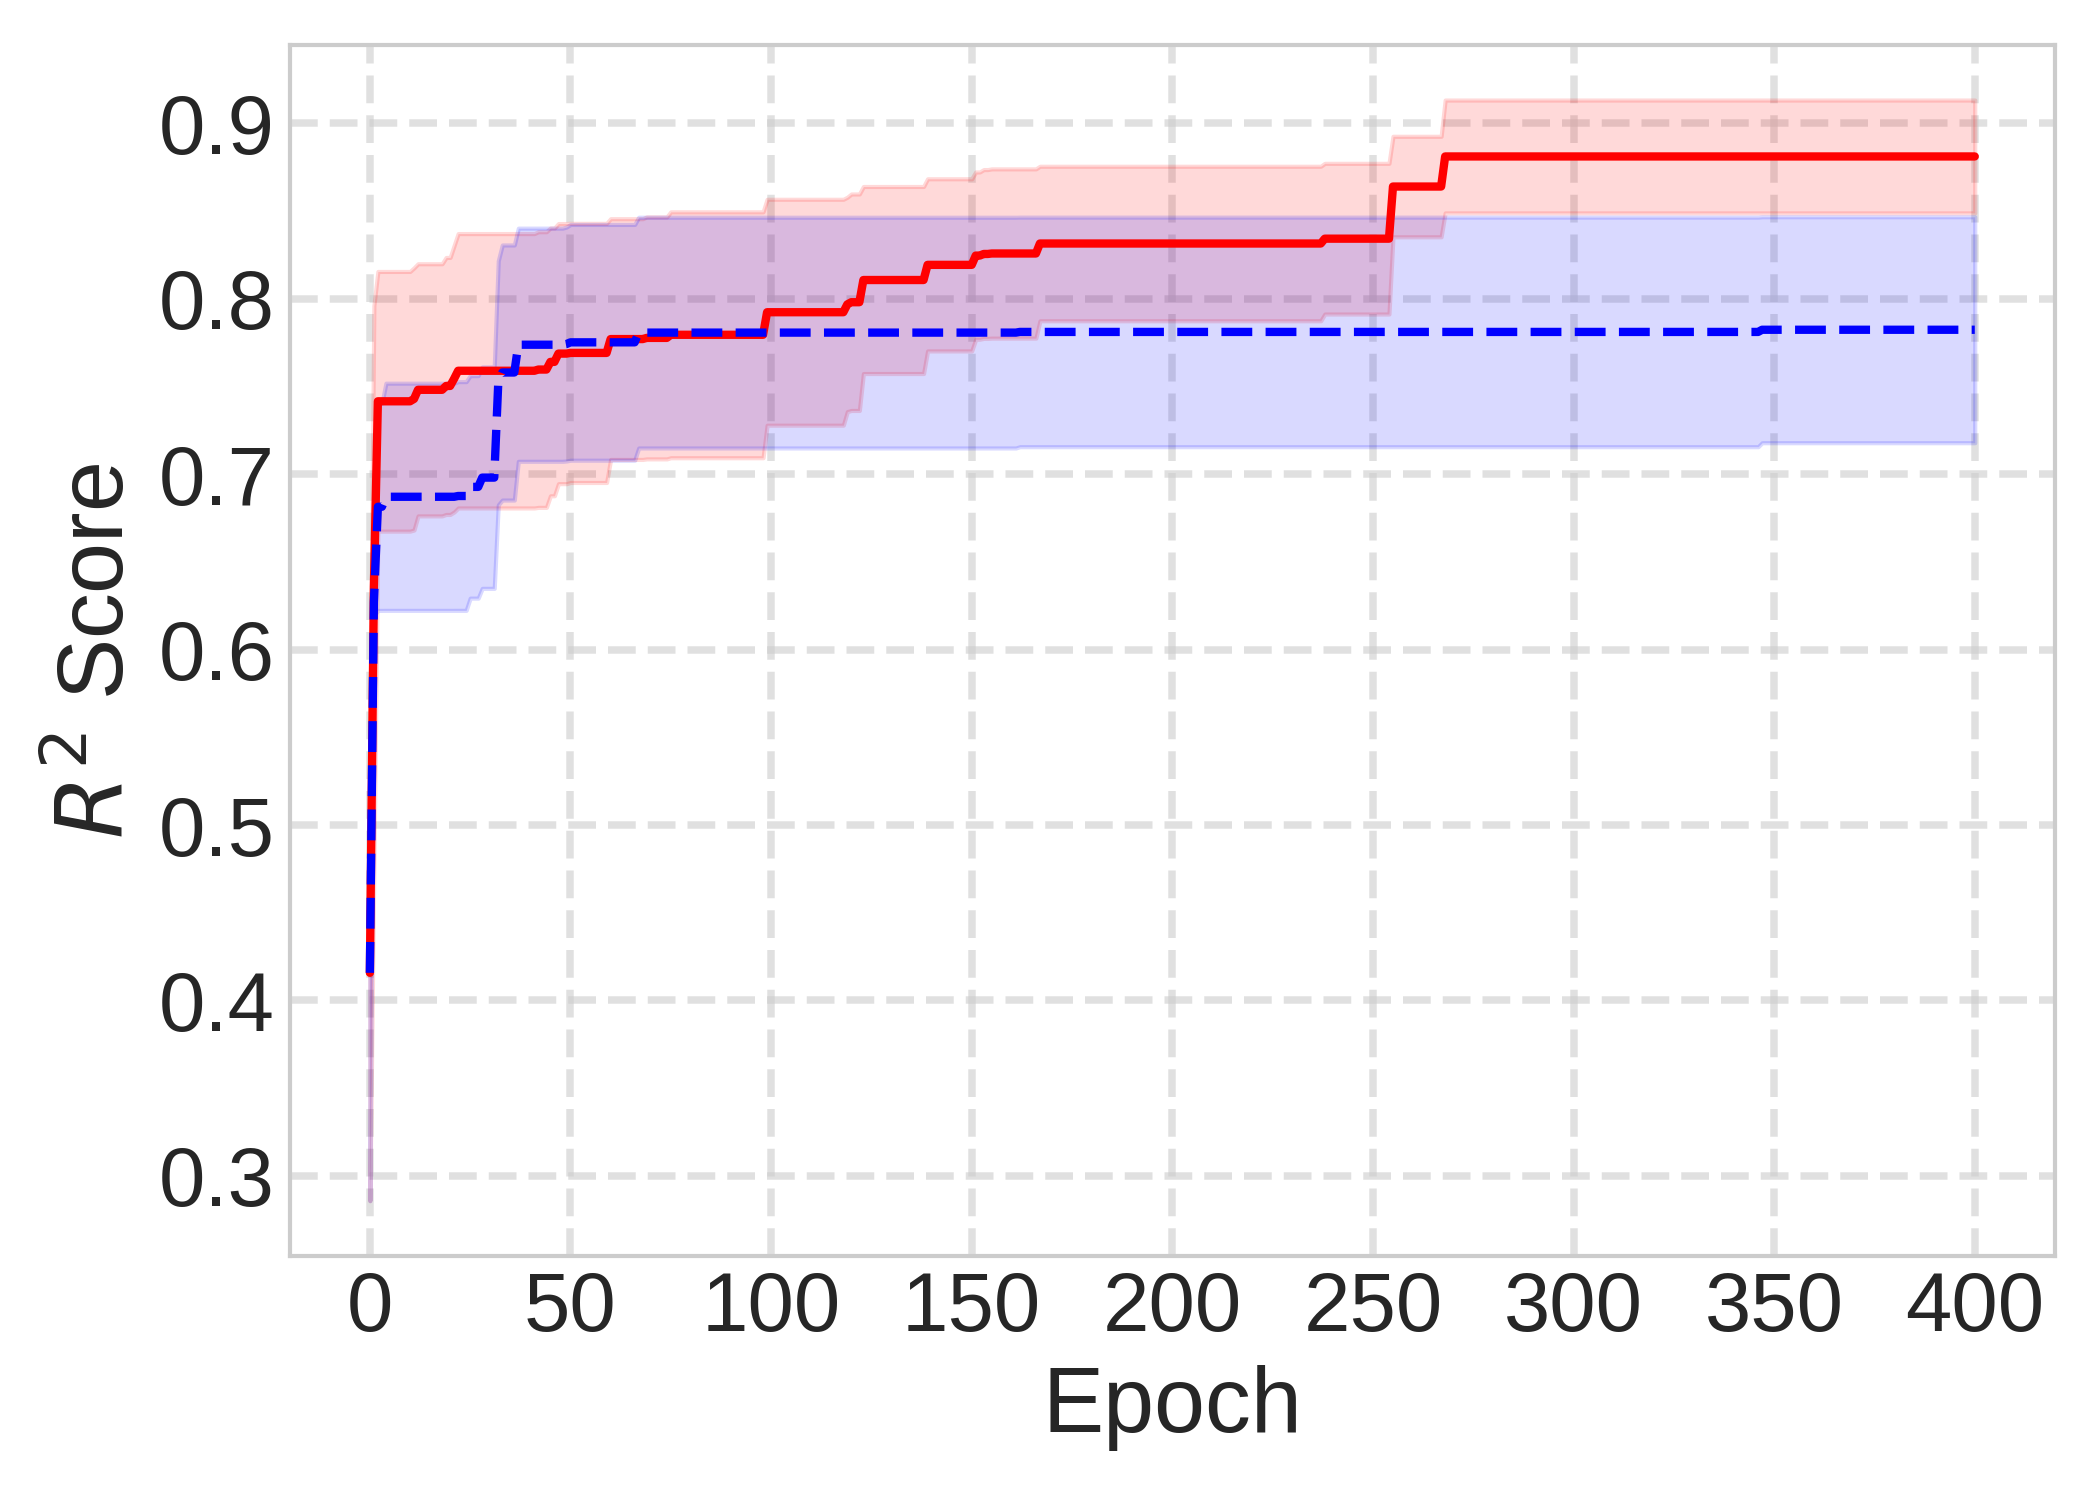
\includegraphics[width=\linewidth]{fig2/Allen_Cahn_testing_r2_v1.png}
  \caption{\small Allen-Cahn}
\end{subfigure}\hfill
\caption{\small Optimization trajectories (test $R^2$) across five PDEs: 
red solid: \textsc{NeuroSym-BO}; blue dashed: Fixed Prompt baseline. 
Shaded regions indicate $\pm$SEM over 5 trials. Our method exhibits 
step-wise improvements from adaptive strategy switching, while the 
baseline plateaus early.}
\label{fig:five-in-a-row}
\end{figure*}






